\documentclass{article}

\usepackage{graphicx}

\usepackage{color}

\usepackage{amsmath, amssymb, amsthm}

\usepackage{float}

\usepackage{caption}
 
\usepackage{algorithmicx, algorithm, algpseudocode}
\floatname{algorithm}{Algorithm}
 
%\usepackage[noline,boxruled,commentsnumbered,linesnumbered,titlenumbered]{algorithm2e}
 
\title{In Grid Multi-Scale Parallel Discrete Element Method for Non-Spherical Particle Dynamics}
\author{
  Konstantinos Krestenitis
  \thanks{
    School of Engineering and Computing Sciences, Durham University,
    DH1 3LE Durham, UK,
    konstantinos.krestenitis@durham.ac.uk
  }
}
\date{\today}

\newcommand{\DeltaSoftware}{\texttt{Delta} $\Delta$}

 \newenvironment{observation}[1][Observation]{\vspace{0.2cm}\noindent\textbf{#1.}\
 }{\vspace{0.2cm}}


\begin{document}
\maketitle

\section{Introduction}

\marginpar{\footnotesize What is DEM. Why does DEM matter (application areas)?}
Lorem ipsum. Lorem ipsum. Lorem ipsum. Lorem ipsum. Lorem ipsum. Lorem ipsum.
Lorem ipsum. Lorem ipsum. Lorem ipsum. Lorem ipsum. Lorem ipsum. Lorem ipsum. 

\marginpar{\footnotesize There are two important shortcomings of many codes:
only spheres and too few of them. Furthermore, many codes suffer if spheres
are of different orders of magnitudes. Why does it make sense to tackle this?}
Lorem ipsum.
Lorem ipsum.
Lorem ipsum. Lorem ipsum. Lorem ipsum. Lorem ipsum.
Lorem ipsum. Lorem ipsum. Lorem ipsum. Lorem ipsum. Lorem ipsum. Lorem ipsum. 

\marginpar{\footnotesize Major objective/contribution of this paper.}
Upscaling a DEM code with respect to particle count and machine size 
challenges the objective to work with triangulated particles from a vast range
of particle sizes.
DEM codes spend a majority of their compute time in collision detection.
\marginpar{\footnotesize Tomek: citation.} 
This phase becomes significantly more complicated if we switch from
sphere-to-sphere checks to the comparison of billions of triangles.
Geometric comparisons suffer from poor SIMDability if realised
straightforwardly.
Multiple contact points between any pair of particles may exist, and it is
impossible to predict statically how this computational workload distributes
between ranks if particles are distributed among ranks. 
The distribution itself is non-trivial if there are particles from a vast range
of scales, which in turn again makes the contact point relation more complicated
than for particle sets of (roughly) the same size.
Finally, the amount of data to be exchanged per particle is higher
than for spherical data where a centre and a radius describe the object of interest. 
The computational work thus increases significantly with any increase of
particle counts.
The scalability of this computational work in turn is not given by construction.
The present paper introduces realisation idioms of a triangle-based DEM code
that fuses efficiency and scalability on all levels of the machine architecture spanning from
vectorisation and memory access characteristics over manycore to inter-node
data exchange.
It shows that the upcoming massively parallel era will allow us to
simulate non-sperical DEM formulations with unpreceded speed.   

\marginpar{\footnotesize What do we do and how does it differ/fit to others'
work?}
Lorem ipsum. Lorem ipsum. Lorem ipsum. Lorem ipsum. Lorem ipsum. Lorem ipsum.
Lorem ipsum. Lorem ipsum. Lorem ipsum. Lorem ipsum. Lorem ipsum. Lorem ipsum. 

\marginpar{\footnotesize Shortcomings and limitations of the present approach.}
Lorem ipsum. Lorem ipsum. Lorem ipsum. Lorem ipsum. Lorem ipsum. Lorem ipsum.
Lorem ipsum. Lorem ipsum. Lorem ipsum. Lorem ipsum. Lorem ipsum. Lorem ipsum. 


- Non-spherical particles reduce efficiency significantly [78,104] in Samiei
- Analytical shape functions besides spheres [41,56,61,118] in Semiei und er
selbst
- Generic shape composition with spheres [75] und Samiei selber


\marginpar{\footnotesize Structure of work.}
The remainder of the paper is organised as follows: 
We start from a brief sketch the overall DEM simulation with
explicit time stepping in Section \ref{section:algorithm}. 
A multiscale grid meta data structure (Section \ref{section:grid}) helps us to
reduce the algorithms complexity to linear.
Starting from this, the main part of the contribution studies a proper data
layout of particle and collision data (Section \ref{section:vectorisation}) that is well-suited for
vectorisation, allows us to exploit multi- and manycore
architectures in various ways (Section \ref{section:shared-memory}) as well as
classic parallel architectures via MPI and domain decomposition (Section
\ref{section:domain-decomposition}).
In Section \ref{section:benchmarks}, we use all algorithmic ingredients to run some benchmarks
that reveal the potential and impact of a technology supporting non-spherical
particles efficiently, before we present performance studies (Section
\ref{section:results}).
A brief summary and an outlook close the discussion.

\input{02_physicalmodel}
\section{Algorithm outline}
\label{section:algorithm}
 
\begin{algorithm}
 
   Blueprint of explicit DEM code's overall structure.
 
 \label{algorithm:dem-blueprint}
% \SetAlgoNoLine
 \begin{algorithmic}[1]
   \For{$t < T$}
   
	\For{i = 0 to N triangles}

		\For {j = i+1 to N triangles}
				
			\State $distance = TTD(i,j)$
				
			\If{(distance $<$ margin) AND ParticleID(i) != ParticleID(j)}

				\State $contact(PID(i)).add(point, normal)$

			\EndIf
			
		\EndFor
			
	\EndFor


	\For{z = 0 to NB particles}

		\For {k = 0 to contacts(z).size()}

			\State $force = granular(velocity(z), position(z), contacts(z).getcontact(k))$

		\EndFor
	
	\EndFor    
    
     \State $t \gets t + \Delta t$
   \EndFor   

 \end{algorithmic}
\end{algorithm} 


We focus on DEM with explicit time stepping (Algorithm \ref{algorithm:dem-blueprint}). 
A straightforward implementation consists of one outer time stepping loop
hosting three inner loops. 
The first inner loop detects contact points between particles' triangles and
check each triangle vs.~the others.
It thus has to loop over the particles.
The second loop runs over these contact points and translates them into forces.
While contact points could in principle be translated into forces straightaway,
it makes sense to outsource the force computation into a separate algorithm
phase.
The third loop applies the forces to the particles and updates the particle
positions.
It has to loop over all particles.


{\bf Contact detection.}
We employ a visco-elastic particle model with spring forces here, where the
actual particle is incompressible.
However, it is equipped with a small halo layer of size $\epsilon >0$:
While the particles are rigid bodies, two particles are assumed to contact each
other if their distance is smaller than $2\epsilon$. 
However, the distance always is positive.
Such an approach equals a Minkowsi sum approach where the actual particles are
blown up by a circle with radius $\epsilon$ and may penetrate each other up to
depth of $\epsilon $.


\begin{figure}[htb]
  \begin{center}
    \includegraphics[width=0.45\textwidth]{sketches/minkowski.pdf}
  \end{center}
  \caption{
    Left: Three particles with their $\epsilon $ environment. The particles do
    not penetrate each other, but two particles plus their $\epsilon $
    environment penetrate and create one contact point with a normal. 
  }
  \label{figure:minkowski}
\end{figure}

As we apply a solid particle model, contact always is a unique point. 
We define it to be the centre of an overlap region (Figure \ref{figure:minkowski}), i.e.~the
distance $d$ between a particle $A$ and its contact point with a second particle
is $0 < d \leq \epsilon$.
Each contact point is equipped with a normal $n$ pointing from the contact point
to the surface of the contacting body's surface.
As the distance is positive, the normal is well-defined and we have $|n| \leq
\epsilon $.
Please note that the normal direction depends on whether we make particle $A$
being hit by particle $B$ or the other way round: each normal associated with a
particle points along the outer normal of the body.
Despite the fact that we employ a rigid body model, multiple contact points
between two bodies may exist as particles may be concave and their Minkowsi sum
may overlap.


For two given particles $A$ and $B$ with corresponding sets of triangles
$\mathbb{T}_A$ and $\mathbb{T}_B$, the contact detection thus reads:
Loop over all triangle pairs $t_i \in \mathbb{T}_A, t_j \in \mathbb{T}_B$ and
identify those pairs that are closer than $2\epsilon $.
For those close, determine the middle point along the closest distance. 
The point equals the contact points while the distance vector identifies
its normal.
Add the contact point to a contact point set $\mathbb{C}_A$ and to the set
$\mathbb{C}_B$.
The normal in the latter is inverted.
Such an algorithm has the complexity $\mathcal{O}( | \mathbb{T}_A| \cdot
|\mathbb{T}_B|)$ and makes the overall naive implementation a member of 
$\mathcal{O}( | \mathbb{T} |_{max}^2  )$ if $| \mathbb{T} |_{max} )$
is the maximum number of triangles per particle.


{\bf Force model.}
We apply the linear spring-dashpot force model from Cundall and
Strack \cite{19,Samiei} to study the efficiency of our implementation.
Per particle $A$, it accumulates all contact points in $\mathbb{C}_A$ into one
translational and one rotational repulsive force with some damping.
We make $\mathbb{C}_A$ subject to a postprocessing which eliminates all
collision point duplicates which is all duplicates that are closer than
$min(h_{A,min},h_{B,min})$. 
It is the smallest face length of the meshes representing $A$ and $B$.
No contact point may be closer than this value.
On the preprocessed contact point set $\mathbb{C}_A$ we then determine
\begin{eqnarray}
%   f_{trans} = \sum _{c \in \mathbb{C}_A} 
%   -k_{repulsive} (\epsilon - |n|) \frac{n}{|n|}
%   \\
  f_{trans} = \sum _{c \in \mathbb{C}_A} 
  \min \left( 0, -k_{repulsive} (\epsilon - |n|) + k_{damp}
  \frac{(v_B-v_A,n)}{|n|}  \right) \frac{n}{|n|}
  \label{equation:forces:translational}
  \\
  f_{rot} = \sum _{c \in \mathbb{C}_A}
  \label{equation:forces:rotational}
\end{eqnarray}

%What are the expensive phases 
\noindent
$k_{repulsive}$ and $k_{damp}$ are material coefficients. 
We use the normal's norm to determine the model's penetration depth, while the
change rate of this depth is derives from the projection of the relative
velocity between the two particles onto the normal vector.
We use the the particles' velocities $v_A$ and $v_B$ here.
The $\min $ function ensures that the force always pulls particle away from each
other. 
There is no particle attraction.


Our Newtonian DEM code relies solely on pair-wise interactions so far. 
With a modifcation of
($\ref{equation:forces:rotational}$,$\ref{equation:forces:rotational}$), it is
however possible to introduce more sophisticated force patterns.
We note that the complexity of the force computation depends solely on the size
of $\mathbb{C}$ if we anticipate that we have to run over all particles to
update their position in space due to momentum anyway.
$\mathbb{C}$ typically is very small if particles are of reasonably the same
size. 
If particle sizes vary dramatically, comparably large particles experience
contact forces from many small particles.
In this case, there are however few large particles compared to the overall
number of particles.


{\bf Time stepping.}
For the present work, we rely on an explicit Euler as simplest time stepping
scheme possible.
We implement a symplectic scheme where the velocity is updated with the forces
before the position is updated with the new velocity \cite{Samiei,37}. 
While the extension to implicit schemes is beyond scope \cite{xxx}, our outlook
does discuss more sophisticated and adaptive time step choices which translate
the present time-driven scheme into an event-driven algorithm \cite{xxx}.


\input{04_algorithm}
\section{Grid meta data structures}
\label{section:grid}

Various speedup techniques such as linked-cell lists \cite{xxx} and Verlet lists
\cite{xxxx} reduce the quadratic complexity in DEM codes.
Notably inspiration in this context stems from the molecular dynamics community
\cite{mattutis:24,wolfgang}. 
In the present paper, we propose to rely on a generalised tree-based linked-cell
technique that allows us to efficiently treat particles of a vast range of diameters.
Three observations support this design decision:
First, particles colliding with other particles are close to these particles.
It thus is sufficient to scan a certain environment around each particle for
potential collision partners.
We do not have to run through all particles per particle.
We thus split up the domain into control volumes.
They are cubic as this simplifies the implementation compared to control volumes
of more flexible shapes.
Second, we may choose these control volumes to be larger than the biggest
particle diameter. 
For a particle held in a particular control volume (cell), it is thus sufficient
to check the $3^d-1$ neighbouring cells whether they host other particles that
might collide. 
$d$ is the spatial dimension.
Third, the previous decision is problematic if the particles are of extremely
different size. 
The cell size is determined by the largest particle diameter. 
If we use a uniform cell size, many uneccessary collision checks are performed
for small particles.
If we use an adaptive grid, it is tricky to design the grid such that only
direct neighbouring cells have to be studied.
We thus, third, observe that a cascade of grids might be useful: If we have
several grids embedded into each other, we can store each particle in the grid
suiting its diameter.
Particles of one grid then have to be checked agains particles in their
neighbouring cell as well as neighbouring cells on coarser grid resolution
levels.
There is no need to check a particle of one grid resolution with particles of a
finer grid resolution---if a particle $A$ collides with a particle $B$, particle
$B$ also collides with particle $A$ and such relations thus are already
detected.


Alternative approaches select the mesh size to accomodate the minimal particle
diameter \cite{mattutis}.
In this case, larger particles overlap multiple cells.
Such an approach requires more sophisticated bookkeeping of particle-cell
relations. 
The idea is not followed up here.
Instead, we prioritise algorithm simplicity---a property that is notably enabled
through trees decomposing the computational domain.


A spacetree is a space-partitioning data structure constructed recursively.
The computational domain is embedded into a unit cube.
We cut the unit cube into three equidistant pieces along each coordinate axis. 
This yields 27 new cubes. 
They are called children of the bounding box cube which is the root.
For each of the children, we continue recursively to evaluate the split
decision. 
The decision to cut into three parts results from the fact that we rely on a
code base based upon three-partitioning \cite{Software:Peano}.
Bipartitioning, i.e.~the classic octree, works as well.


The construction scheme yields a cascade of ragged regular Cartesian grids that
are embedded into each other.
Each cell besides the root has a unique parent cell.
While we could make the cells hold particles, we propose to use a
multiscale, vertex-based scheme spanning a dual meta grid
\cite{Weinzierl:16:PIC}.
A vertex is unique through its spatial position plus its level. 
The level is the number of refinement steps required at least to create one of
its adjacent cells.
Each vertex holds a list of particles.
A particles is always stored on the finest grid level where the cells' edge
length is still bigger than its diameter.
A particle is always associated to the vertex next to its geometric centre,
i.e.~any vertex has a list of all particles close to it on the same level.
Links from the vertices to the particles are realised as pointers. 
If a particle moves, we have to update the links, but we do not move
geometric data in memory.


\input{05a_grid-traversal}



{\bf Regular grid.}
The spacetree formalism allows us to realise at least three grid variants. 
A very simple refines all spacetree nodes all the time as long as the resulting
cell mesh size is bigger than the largest particle diameter.
Such a strategy yields a regular Cartesian grid. 

\input{05b_adaptive-grid}

\input{06_vectorisation}
\input{07_shared-memory}
\input{08_distributed-memory}
\input{09_casestudies}
\input{10_conclusion}
\input{11_acknowledgements}
\input{12_appendix}

\bibliographystyle{plain}
\bibliography{./paper}

\appendix

\section{Software}
\label{section:software}

All underlying software is free and open source C++ code.
\DeltaSoftware\ is available from \cite{Software:Delta} and offers all the
functionality introduced in Section \ref{section:vectorisation} through
\ref{section:domain-decomposition}.
All spacetree and adaptive mesh refinement routines (Section ref{section:grid}) used in the
present work rely on the framework Peano
\cite{Software:Peano,Weinzierl:2009:Diss,Weinzierl:11:Peano}.
All geometric operations as well as DEM-specific compute kernels however are
independent of Peano and can be used with any other (spacetree-based) software.

We offer \DeltaSoftware\ with single (\texttt{float}) and double
(\texttt{double}).
The accuracy is controlled via a compile flag \texttt{-DiREAL=}.
Subject of study here is exlusively \texttt{double}. 
Studies on reduced accuracy computations are beyond the scope of the present
work.

\section{Experiment: Two particles}
\label{section:experiment:two-particles}

The present experiments study two particles that bump into each other and then
move away because of the spring dashpot forces.
The two particles are represented by 126 triangles. 
We simulate 15,000 time steps.
A contact is detected first in iteration 9,541 and introduces a force making the
two particles to move away from each other. 
The code however still needs another 5 iterations to make the particles be away
from each other more than $\epsilon=10^{-4}$.
If the two particles are compared, this results in 3,944 triangle-triangle
comparisons.
 
The experiments can be rerun with 
{\footnotesize
\begin{verbatim}
./dem-3d-asserts 0.3 0.1 0.02 two-particles-crash 15000 regular-grid 0.0001 \ 
upon-change 0.0

./dem-3d-asserts 0.3 0.1 0.02 two-particles-crash 15000 adaptive-grid 0.0001 \
upon-change 0.0

./dem-3d-asserts 0.3 0.1 0.02 two-particles-crash 15000 reluctant-adaptive-grid \
0.0001 upon-change 0.0
\end{verbatim}
}

{\bf Regular grid.} We obtain a grid with 1,032 vertices. The first 6,334
iterations, we do not perform any contact detection. The subsequent grid
traversals perform all 3,944 comparisons till iteration 12,503. Starting from
time step 12,504, the particles are far away from each other again and we do not
compare anything anymore.

\begin{center}
  \includegraphics[width=0.3\textwidth]{experiments/two-bodies/visualisation/regular-grid00.png}
  \includegraphics[width=0.3\textwidth]{experiments/two-bodies/visualisation/regular-grid01.png}
  \includegraphics[width=0.3\textwidth]{experiments/two-bodies/visualisation/regular-grid02.png}
\end{center}


{\bf Adaptive grid.} We obtain a grid with 747 vertices. Only few iterations
(when one particle enters a neighbouring region) make the number increase to
980, but these grids are immediately after reduced to 747 again.
The first 8,556 iterations, we do not perform any contact detection. The
subsequent grid traversals perform all 3.944 comparisons.
In iteration 9,539 we detect contact and the particles start to move away
from each other, but we continue to check for further contacts till iteration
10,415.
From here on, the particles are far away from each other again
and we do not compare anything anymore.

% \begin{center}
%   \includegraphics[width=0.3\textwidth]{experiments/two-bodies/visualisation/adaptive-grid00.png}
%   \includegraphics[width=0.3\textwidth]{experiments/two-bodies/visualisation/adaptive-grid01.png}
%   \includegraphics[width=0.3\textwidth]{experiments/two-bodies/visualisation/adaptive-grid02.png}
% \end{center}


{\bf Reluctant adaptive grid.} The reluctant adaptive grid behaves qualitatively
similar to the plain adaptive grid though yields quantitatively a smaller number
of vertices. 
We start from a grid with 498 vertices, i.e.~we do not refine the grid down to
the same fine level as the adaptive approach.
In iteration 6,334, both particles enter the same coarse grid cell and we run
3,944 triangle-triangle comparisions. 
They yield no contact yet.
The reluctant criterion refines the grid that has now 980 vertices starting from
iteration 6,338 on.
The code continues to run without any further comparisons till iteration 8,556
when the particles again are close to each other (close this time w.r.t.~finest
grid level allowed by the particle diameters).
Between iteration 8,557 and 9,533 we continue to run with 980 vertices and
3,944 comparisons.
The code decides to reduce the grid in iteration 9,536 to 747 vertices when the
particles are approach each other within a single cube that is resolved with a
fine grid.
We detects contact in iteration 9,541 after which the particles move away from
each other.
The 747 vertices are preserved and the code continues to run 3,944 comparisons.
In iteration 10,452, the particles are far away from each other. 
No more comparisons are performed from hereon.
In iteration 14,556 the particles are far away from each other, leave the
fine tessellation around the previous contact point and we continue with a
coarser grid of 498 vertices.

%  \begin{center}
%   \includegraphics[width=0.3\textwidth]{experiments/two-bodies/visualisation/reluctant-adaptive-grid00.png}
%   \includegraphics[width=0.3\textwidth]{experiments/two-bodies/visualisation/reluctant-adaptive-grid01.png}\\
%   \includegraphics[width=0.3\textwidth]{experiments/two-bodies/visualisation/reluctant-adaptive-grid02.png}
%   \includegraphics[width=0.3\textwidth]{experiments/two-bodies/visualisation/reluctant-adaptive-grid03.png}\\
%  \end{center}

\section{Experiment: Some comparison statistics}
\label{section:experiment:comparison-statistics}

\begin{center}
  \includegraphics[width=1\textwidth]{experiments/random/no-of-collisions/grid.png}
\end{center}

\begin{center}
 	\includegraphics[width=1\textwidth]{experiments/random/no-of-collisions/adaptive.png}
\end{center}

\begin{center}
  \includegraphics[width=1\textwidth]{experiments/random/no-of-collisions/reluctant.png}
\end{center}

\begin{center}
  \includegraphics[width=1\textwidth]{experiments/random/no-of-collisions/gridG.png}
\end{center}

\begin{center}
  \includegraphics[width=1\textwidth]{experiments/random/no-of-collisions/adaptiveG.png}
\end{center}

\begin{center}
  \includegraphics[width=1\textwidth]{experiments/random/no-of-collisions/reluctantG.png}
\end{center}

\section{Randomised particle generation}
\label{section:randomised-particle-generation}

For our particle generation, we rely on the convex hull algorithm
\cite{mattutis,3,5}.
We place 50 points random on the unit sphere
They act as input to the computation of a convex hull which yields around 60
triangles typically.
Each vertex of the resulting mesh then is scaled with a random scalar from
$[0.75,1]$.
Thus, we obtain distorted particles that do not resemble a sphere and can be
slightly convex.
The resulting mesh is finally suitably dilated and scaled.

\begin{figure}[htb]
  \begin{center}
    \includegraphics[width=0.5\textwidth]{sketches/coarse.png}
  \end{center}
  \caption{Coarse non-spherical particle triangulation using Hull and Delaney algorithm.}
  \label{figure:coarse_particle}
\end{figure}

\begin{figure}[htb]
  \begin{center}
    \includegraphics[width=0.5\textwidth]{sketches/coarse.png}
  \end{center}
  \caption{Fine spherical particle triangulation using Hull and Delaney algorithm.}
  \label{figure:fine_particle}
\end{figure}


\marginpar{\footnotesize KK: Can you please add here two or three pictures from
typical particles?}


\end{document}
